\documentclass{standalone}
\usepackage[T1]{fontenc}
\usepackage[latin2]{inputenc}
\usepackage[english]{babel}
\usepackage{tikz}
\usetikzlibrary{calc,through,backgrounds,positioning,fit}
\usetikzlibrary{shapes,arrows,shadows}
 
\begin{document}
 
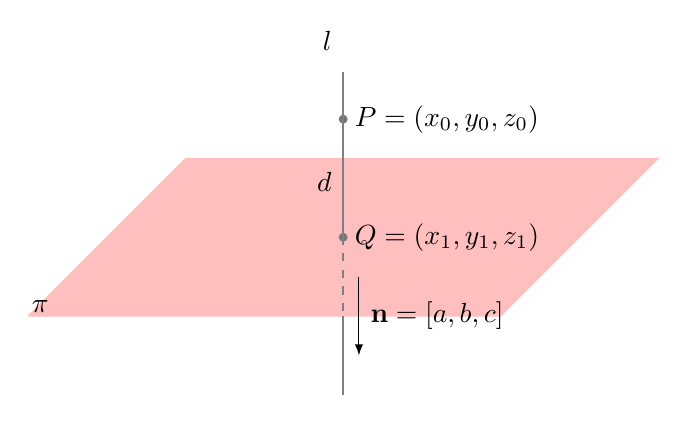
\begin{tikzpicture}[scale=1,inner sep=0.4mm]

\draw [pink, fill=pink] (0,0)--(6,0) -- (8,2) -- (2,2)--(0,0); 

\draw [gray, fill=gray!90!black] (4,1) circle (0.05cm);
\draw [gray, fill=gray!90!black] (4,2.5) circle (0.05cm);

\draw [gray, thick] (4.0,3.1)--(4.0,0.9);
\draw [gray, thick, dashed] (4.0,0.8)--(4.0,0);
\draw [gray, thick] (4.0,0.0)--(4.0,-1);
\draw [-latex] (4.2, 0.5)--(4.2, -0.5); 

\node at (4.1,1) [right]{$Q=(x_{1}, y_{1}, z_{1})$}; 
\node at (4.1,2.5) [right]{$P=(x_{0}, y_{0}, z_{0})$};
\node at (3.9,3.5) [left]{$l$};
\node at (3.9,1.7) [left]{$d$};
\node at (0,0) [above right]{$\pi$};
\node at (4.3,0) [right]{$\textbf{n} =[a,b,c]$};

\end{tikzpicture}
 
\end{document}